\RequirePackage[abort, l2tabu, orthodox]{nag}
\documentclass[pageno]{jpaper}

% standard LaTeX packages that do not interfere with hyperref
\usepackage{alltt}
\usepackage{amssymb}
\usepackage{booktabs}
\usepackage{caption}
\usepackage[draft]{fixme}
\usepackage{epstopdf}
\usepackage{flushend}
\usepackage{graphicx}
\usepackage[final]{listings}
\usepackage[sort&compress]{natbib}
\usepackage{paralist}
\usepackage{tikz}
\usepackage[normalem]{ulem}
\usepackage{xspace}

% font selection
\usepackage{courier}
\usepackage{helvet}
\usepackage{mathptmx}
\usepackage{microtype}
\usepackage[mathscr]{euscript}

% hyperref itself
\usepackage{hyperref}

% standard packages that must be loaded after hyperref
\usepackage{bookmark}
\usepackage{verbatim} 

% should be loaded after listings and subfig
\usepackage{cleveref}
\usepackage{multirow}
\usepackage{enumitem}
\usepackage{xfrac}

% custom packages for this paper
 
\DeclareCaptionType{copyrightbox}

\renewcommand{\cite}[1]{%
  \PackageError{natbib}{%
    The \string\cite\space{} command is ambiguous; use
    \string\citet\space{} or \string\citep\space{} instead}{}}

\renewcommand{\autoref}[1]{%
  \PackageError{cleveref}{%
    Do not use \string\autoref.  Use \string\cref instead, or use
    \string\crefrange for ranges of referenced items}}

\renewcommand{\hline}[1]{%
  \PackageError{booktabs}{%
    Do not use \string\hline.  Use \string\toprule, \string\midrule,
    or \string\bottomrule\space instead depending on where in the
    table the line appears}}

\newcommand{\email}[1]{\href{mailto:#1@univ.edu}{#1}}

% cleveref configuration
\crefname{figure}{Figure}{Figures}
\crefname{section}{Section}{Sections}
\crefname{table}{Table}{Tables}

\hyphenation{test-case}

% lst configuration
\lstdefinelanguage{example}{%
  morekeywords={xyz},
}

\lstset{
  basicstyle=\sffamily,
  columns=fullflexible,
  numbersep=5pt,
  numberstyle=\scriptsize,
  showstringspaces=false,
  language=example,
  escapeinside={/*@}{@*/},
  belowcaptionskip=1\baselineskip,
  language=C,
  showstringspaces=false,
  keywordstyle=\bfseries,
  commentstyle=\itshape,
}


\urlstyle{sf}

\pdfpagewidth=8.5in
\pdfpageheight=11in


% Custom commands
\newcommand{\Tool}{\textsc{XYZ}\xspace}

\sloppy
% start doc
\begin{document}

\title{Title}

\author{a1 a2\\ \email{a1} \email{a2} \\ univ}

\date{}
\maketitle


\begin{abstract}
Abstract goes here
\end{abstract}

\section{Introduction}
\label{sec:intro}

Introduction goes here


\section{Common Stuff}
\label{sec:common}

Refer a paper \citep{Lamport86} or a misc article \citep{lcommon}.\\

Here's a table \cref{tab:tcommon}.\\

\begin{table}
\centering
\small{
  \centering
  \begin{tabular}{rl} \toprule
   {A}& B  \\  
   \cmidrule(lr){1-2}
   a1  & b1  \\ 
   \midrule
   a2  & b2 \\
   \bottomrule
   \end{tabular}
 }
%\nocaptionrule
\caption{Generic caption.}
\label{tab:tcommon}
\end{table}

A multi-column table is show in \Cref{tab:tcommon2}.\\

\begin{table}
  \centering
  \begin{tabular}{lcccc}
    \toprule
    Id & \multicolumn{4}{c}{Big column} \\
      \cmidrule(lr){2-3} \cmidrule(lr){4-5} 
             & A1   &  A2    & B1 & B2  \\ 
      \midrule                       
      row1   & a1   &  a2    & b1 & b2  \\
 \bottomrule
\end{tabular}
%  \nocaptionrule
\caption{Results from tool \Tool}
\label{tab:tcommon2}
\end{table}


Source code is shown in \Cref{fig:codecommon}.

\lstset{basicstyle=\ttfamily\fontsize{9}{10}\selectfont,
   morekeywords={if,else,end}, numbers=left} 
\begin{figure}
\subfloat[\label{fig:codecommon1}]{\parbox[t]{0.22\textwidth}{\lstinputlisting{figure/tmp1.c}}} %
\subfloat[\label{fig:codecommon2}]{\parbox[t]{0.22\textwidth}{\lstinputlisting{figure/tmp2.c}}}
\caption{Code caption.}
\label{fig:codecommon}
\end{figure}

An equation is shown in \Cref{eqn:ecommon}.

\begin{equation}    
\mathrm{x = \frac{\displaystyle |y|}{\displaystyle |z|}}
\label{eqn:ecommon}
\end{equation}

A figure is shown in \Cref{fig:fcommon}.

\begin{figure}[h!]
  \centering
  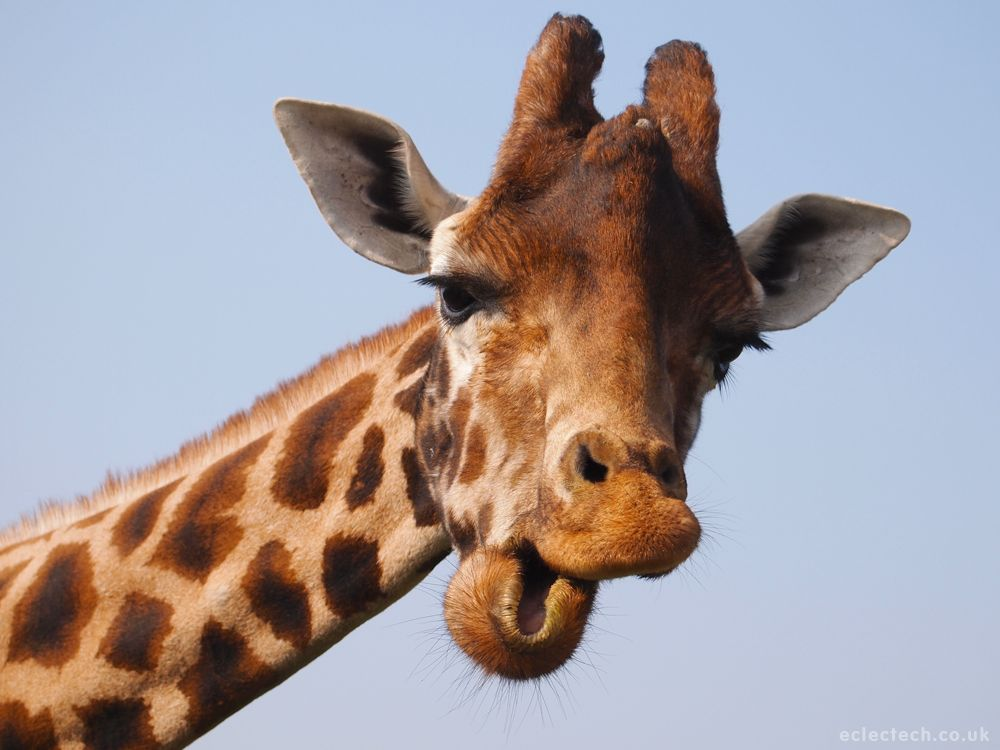
\includegraphics[width=0.3\textwidth]{figure/giraffe.jpg}
  \caption{A picture.}
  \label{fig:fcommon} 
\end{figure}


\bibliographystyle{plain}
\bibliography{ref}

\end{document}
% end doc
